\section{Presentazione del modello di business}

Analizzando il settore e il nostro target di mercato, siamo giunti alla conclusione che il modo migliore per la vendita del prodotto, sia quello di rivolgerci direttamente al cliente finale, vendendo il prodotto prevalentemente online.\\Per questo prevediamo la realizzazione di un \textit{e-commerce} per la vendita diretta al cliente e, in un primo periodo, l'utilizzo di piattaforme già note come \textit{Amazon} per far conoscere ancora di più il nostro prodotto. Sempre online, prevediamo di vendere il prodotto su alcuni e-commerce selezionati e specializzati nella vendita di piante e accessori per quest'ultime, così da raggiungere un segmento di mercato non raggiungibile mediante i canali sopra citati.

\subsection{Collaborazioni}

Non mancheranno alcune collaborazioni mirate insieme ad aziende già presenti nel settore. Ad esempio, prevediamo di intraprendere delle partnership per la vendita di \textit{bundle vaso+PotNet} con aziende che hanno come business principale la realizzazione di vasi eco sostenibili. Tra queste abbiamo:
\begin{itemize}
	\item \textbf{Tera: } azienda giovane ed italiana che produce vasi composti al 100\% da plastica riciclabile e riciclata;
	\item \textbf{Verti Copenhagen: } azienda danese che produce porta-piante per soluzioni verticali, realizzati attraverso l'uso di bucce di patate e altri residui vegetali;
	\item \textbf{Ecopots: } brand scandinavo che utilizza plastica riciclata per la realizzazione di vasi dal design accattivante e durevoli nel tempo;
\end{itemize}


\subsection{Vendita al dettaglio e abbonamenti}

I costi di produzione stimati per singola unità, considerando solo i materiali, saranno compresi tra i 5 e gli 8 euro, con un prezzo di vendita ipotizzato tra i 25 e i 30 euro. \\Dopo alcuni mesi dalla commercializzazione del primo prodotto, prevediamo di commercializzare anche una versione di PotNet con un numero di sensori maggiore. Questo, a fronte di un costo di produzione di poco maggiore (2-3€), ci permetterà di vendere questa nuova versione ad un prezzo tra i 35 e i 40 euro, quindi con un utile superiore rispetto alla prima versione.
\newline\newline Oltre alla semplice vendita del prodotto, saranno presenti dei piani di abbonamento a cui gli utenti potranno sottoscriversi per ottenere funzionalità aggiuntive sul bot Telegram e sulla Web UI; come consigli periodici da parte di esperti del settore, un algoritmo migliorato per l'analisi dei dati e accesso anticipato agli aggiornamenti e alle nuove funzionalità:
\begin{itemize}
	\item Mensile [3.99€]
	\item Trimestrale [10.99€]
	\item Annuale [34.99€]
\end{itemize}

\begin{figure}[ht!]
	\centering
	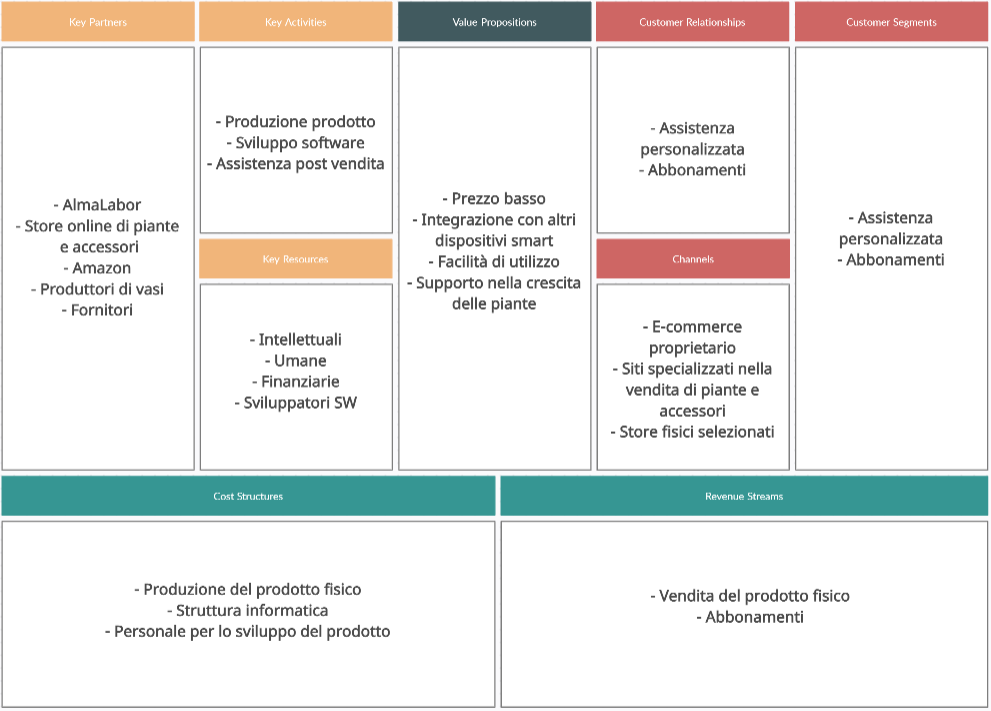
\includegraphics[width=\textwidth]{./images/Business-Model-Canvas.PNG} 
	\caption{Business Model Canvas \label{overflow}}
\end{figure}

\subsection{Pubblicità}

Per aumentare la visibilità del prodotto al lancio, e far conoscere la nostra azienda, puntiamo ad una forte presenza sui maggiori canali social (Instangram, Facebook, TikTok) il nostro cliente tipo è solitamente presente su almeno uno di esso. Invieremo inoltre alcune unità di prova a content creator selezionati per far provare il nostro prodotto, in modo da ricevere alcuni feedback per miglioramenti futuri e ulteriore visibilità sui loro canali.

Il nostro modello di business si basa quindi sui ricavi provenienti dalla vendita del prodotto e dalla sottoscrizione dei clienti agli abbonamenti aggiuntivi proposti. In questo modo uniamo il classico modello in cui la vendita del prodotto fisico rappresenta la maggior parte delle entrate, ad un modello in cui una funzionalità sviluppata una sola volta, continua a generare un profitto per vari mesi e/o anni.

\subsection{Commercializzazione}

Inizieremo commercializzando il prodotto in Europa per poter gestire più facilmente la sua distribuzione e l'assistenza post vendita. Inoltre, ci permetterà di risparmiare anche nello sviluppo software in quanto saranno necessari un numero minore di server e di lingue supportate.\newline Una volta raggiunto un buon numero di clienti e una maggiore solidità finanziaria, procederemo ad analizzare su quali altri mercati commercializzare il prodotto.